\documentclass[25pt, a0paper, portrait, margin=0mm, innermargin=20mm,
blockverticalspace=2mm, colspace=20mm, subcolspace=0mm]{tikzposter} %Default values for poster format options.

\input{packages}

\definecolor{unired}{HTML}{a51e37}
\definecolor{mypink1}{rgb}{0.858, 0.188, 0.478}
\definecolor{mblack}{HTML}{0d0d0d}
\definecolor{titlecolor}{RGB}{74, 114, 159}
\definecolor{titledarkcolor}{RGB}{51,102,153}
\definecolor{Grey}{HTML}{e1e1e1}
\definecolor{DarkerGrey}{RGB}{215,217,219}
\definecolor{FontColor}{HTML}{0d0d0d}
\definecolor{Red}{RGB}{204,0,0}
\definecolor{L-lig}{RGB}{25,124,192}
\definecolor{point-lig}{RGB}{255,255,255}
\definecolor{G-lig}{RGB}{62,66,68}

\definecolor{Orange}{RGB}{240,163,10} 
\definecolor{LightRed}{RGB}{214,98,93}
\definecolor{LightBlue}{RGB}{160,200,217}
\definecolor{LightGreen}{RGB}{130,161,119}
\definecolor{Violet}{RGB}{190,144,252}

\colorlet{blocktitlefgcolor}{mblack}
\colorlet{backgroundcolor}{Grey}
\colorlet{blocktitlebgcolor}{Grey}
\colorlet{blockbodyfgcolor}{FontColor}
\colorlet{innerblocktitlebgcolor}{L-lig}
\colorlet{innerblocktitlefgcolor}{white}
\colorlet{notefrcolor}{white}
\colorlet{notefgcolor}{black}
\colorlet{notebgcolor}{white}




\begin{document}
 
\renewcommand{\baselinestretch}{1} 
\title{\parbox{1500pt}{Color-blindness of direction-selective units in the \\ zebrafish optic tectum}}
\author{Alexander Wendt, Patrick Weygoldt}
\institute{Supervisor: Aristides Arrenberg, Tim Hladnik, David Burkardt}
\usetitlestyle[]{sampletitle}
\maketitle
\renewcommand{\baselinestretch}{1.4} 

\begin{columns}
\column{0.3333}
\myblock[MyBlock]{Introduction}{
   Chromaticity has a big influence on motion vision in zebrafish. 
   Orger and Baier (2004) used the optomotor response to show that combinations of green and red can be used to null the motion perception.
   \vspace{0.7cm}
   \begin{tikzfigure}[]
    \label{Raw}
    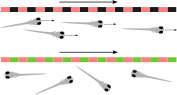
\includegraphics[width=17cm]{figs/omr.pdf}
    \end{tikzfigure} 
   
   But little is known about the midbrain structures conveing the
   \glqq color-motion\grqq{} perception. We investigated the 
   activity of direction-selective units in the optic tectum of zebrafish in response to gratings of various color contrasts using a combination of two-photon microscopy and calcium imaging. 
}
\myblock[MyBlock]{Preprocessing:}{
    \textbf{1. Region of Interests (ROI):}
    corresponds to neurons with genetically encoded calcium indicators. The fluorescence $F$ of the calcium imaging is calculated from the change of luminance normalized to the average luminance $F = \frac{\Delta F}{\langle F \rangle}$.
    
    \vspace{0.5cm}
    \begin{tikzfigure}[]
        \label{Raw}
        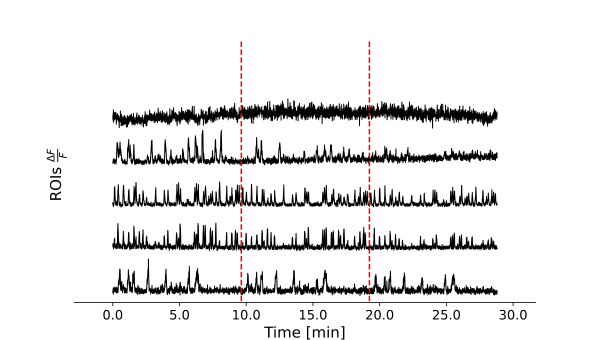
\includegraphics[width=22cm]{figs/autocorrelation.pdf}
    \end{tikzfigure} 
    \vspace{0.6cm}
    \textbf{2. Active ROIs:} Strongly autocorrelated ROIs across stimulus repeats are \glqq responding\grqq{}

        \begin{tikzfigure}[]
            \label{Rois}
            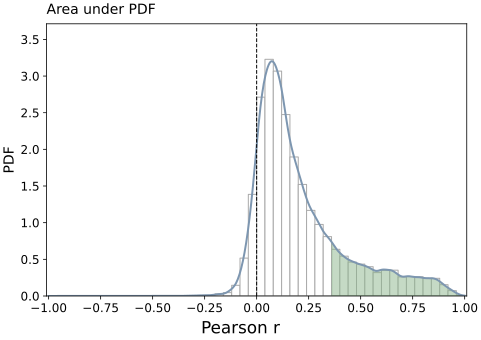
\includegraphics[width=12cm]{figs/pcorrelation.pdf} 
        \end{tikzfigure}
    
    \vspace{0.5}

    \textbf{3. Direction-selective ROIs:} ROIs that correlated with a direction regressor (clockwise (CW) or counterclockwise (CCW)).
    \vspace{-1.3cm}
    \begin{tikzfigure}[]
        \label{Rois}
        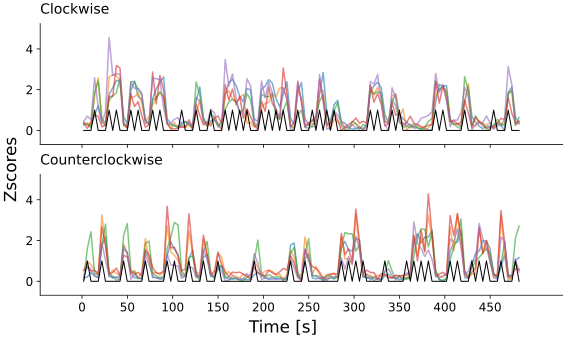
\includegraphics[width=24cm]{figs/regressor.pdf}
    \end{tikzfigure}
}  
\column{0.6666}
\myblock[MyBlock]{2-photon calcium imaging}{
    \vspace{-1.7cm}
    \begin{tikzfigure}[]
        \label{modulations}
        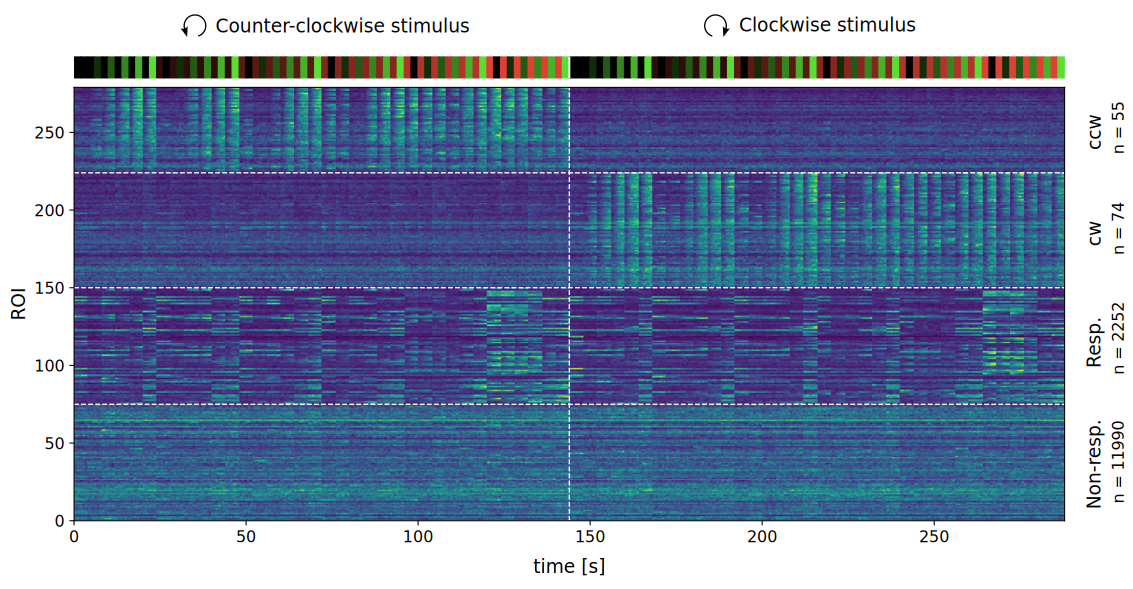
\includegraphics[width=\linewidth]{figs/testimg.pdf
        }
    \end{tikzfigure}

    \begin{tikzfigure}[]
        \label{Raw}
        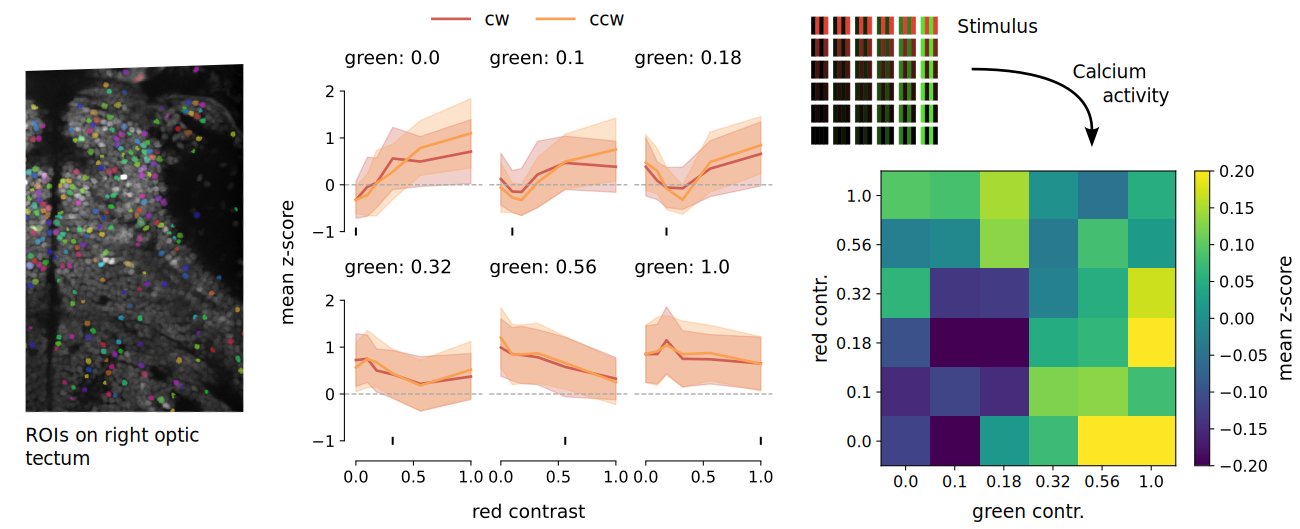
\includegraphics[width=50cm]{figs/contrast_curves_ca.pdf}
    \end{tikzfigure}

    \begin{itemize}
        \item ROIs responded to moving gratings of red and green 
        \item Both directions CW and CCW responded equally 
        \item If both red and green had the same contrast the response was supressed indicating color blindness
        \item A slight shift in the troughs of activity could be explained by a higher intensity of green compared to red.
    \end{itemize}
}   
\myblock[MyBlock]{Behavior}{
    \vspace{-1.7cm}
    \begin{tikzfigure}[]
        \label{Raw}
        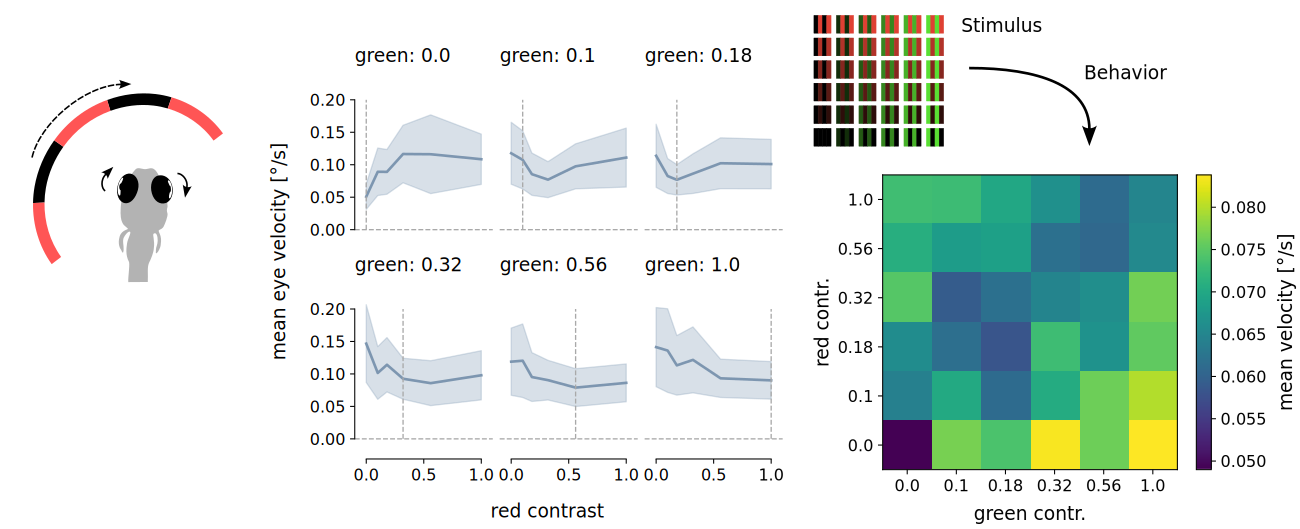
\includegraphics[width=50cm]{figs/contrast_curves_behav_test.pdf}
    \end{tikzfigure}
    \begin{itemize}
        \item The behavioral response (OKR) reflect the pattern shown in calcium activity.
    \end{itemize}
}
\myblock[MyBlock]{Conclusion}{
    \begin{itemize}
        \setlength\itemsep{0.5cm}
        \item We observed that the optic tectum lack the response to red-green merged out-of-phase stimuli and is therefore color-blind
    \end{itemize}
    \vspace{0.2cm}
    }
\end{columns}

%\node [above right, text=white, outer sep=45pt,minimum width=\paperwidth, align=center, draw, fill=unired, color=unired] at (-43.6,-61) { \textcolor{white}{\normalsize Contact: patrick.weygoldt@student.uni-tuebingen.de}};

\end{document}